\columnbreak
\section{Serien- und Parallelschaltung von Zellen und Modulen}
\textcolor{red}{$U_{\mathrm{LL}}$ ändert bei Verschattung nur minimal! Änderung fast nur an $I_{\mathrm{K}}$.}

\subsection{Serienschaltung von Solarzellen}
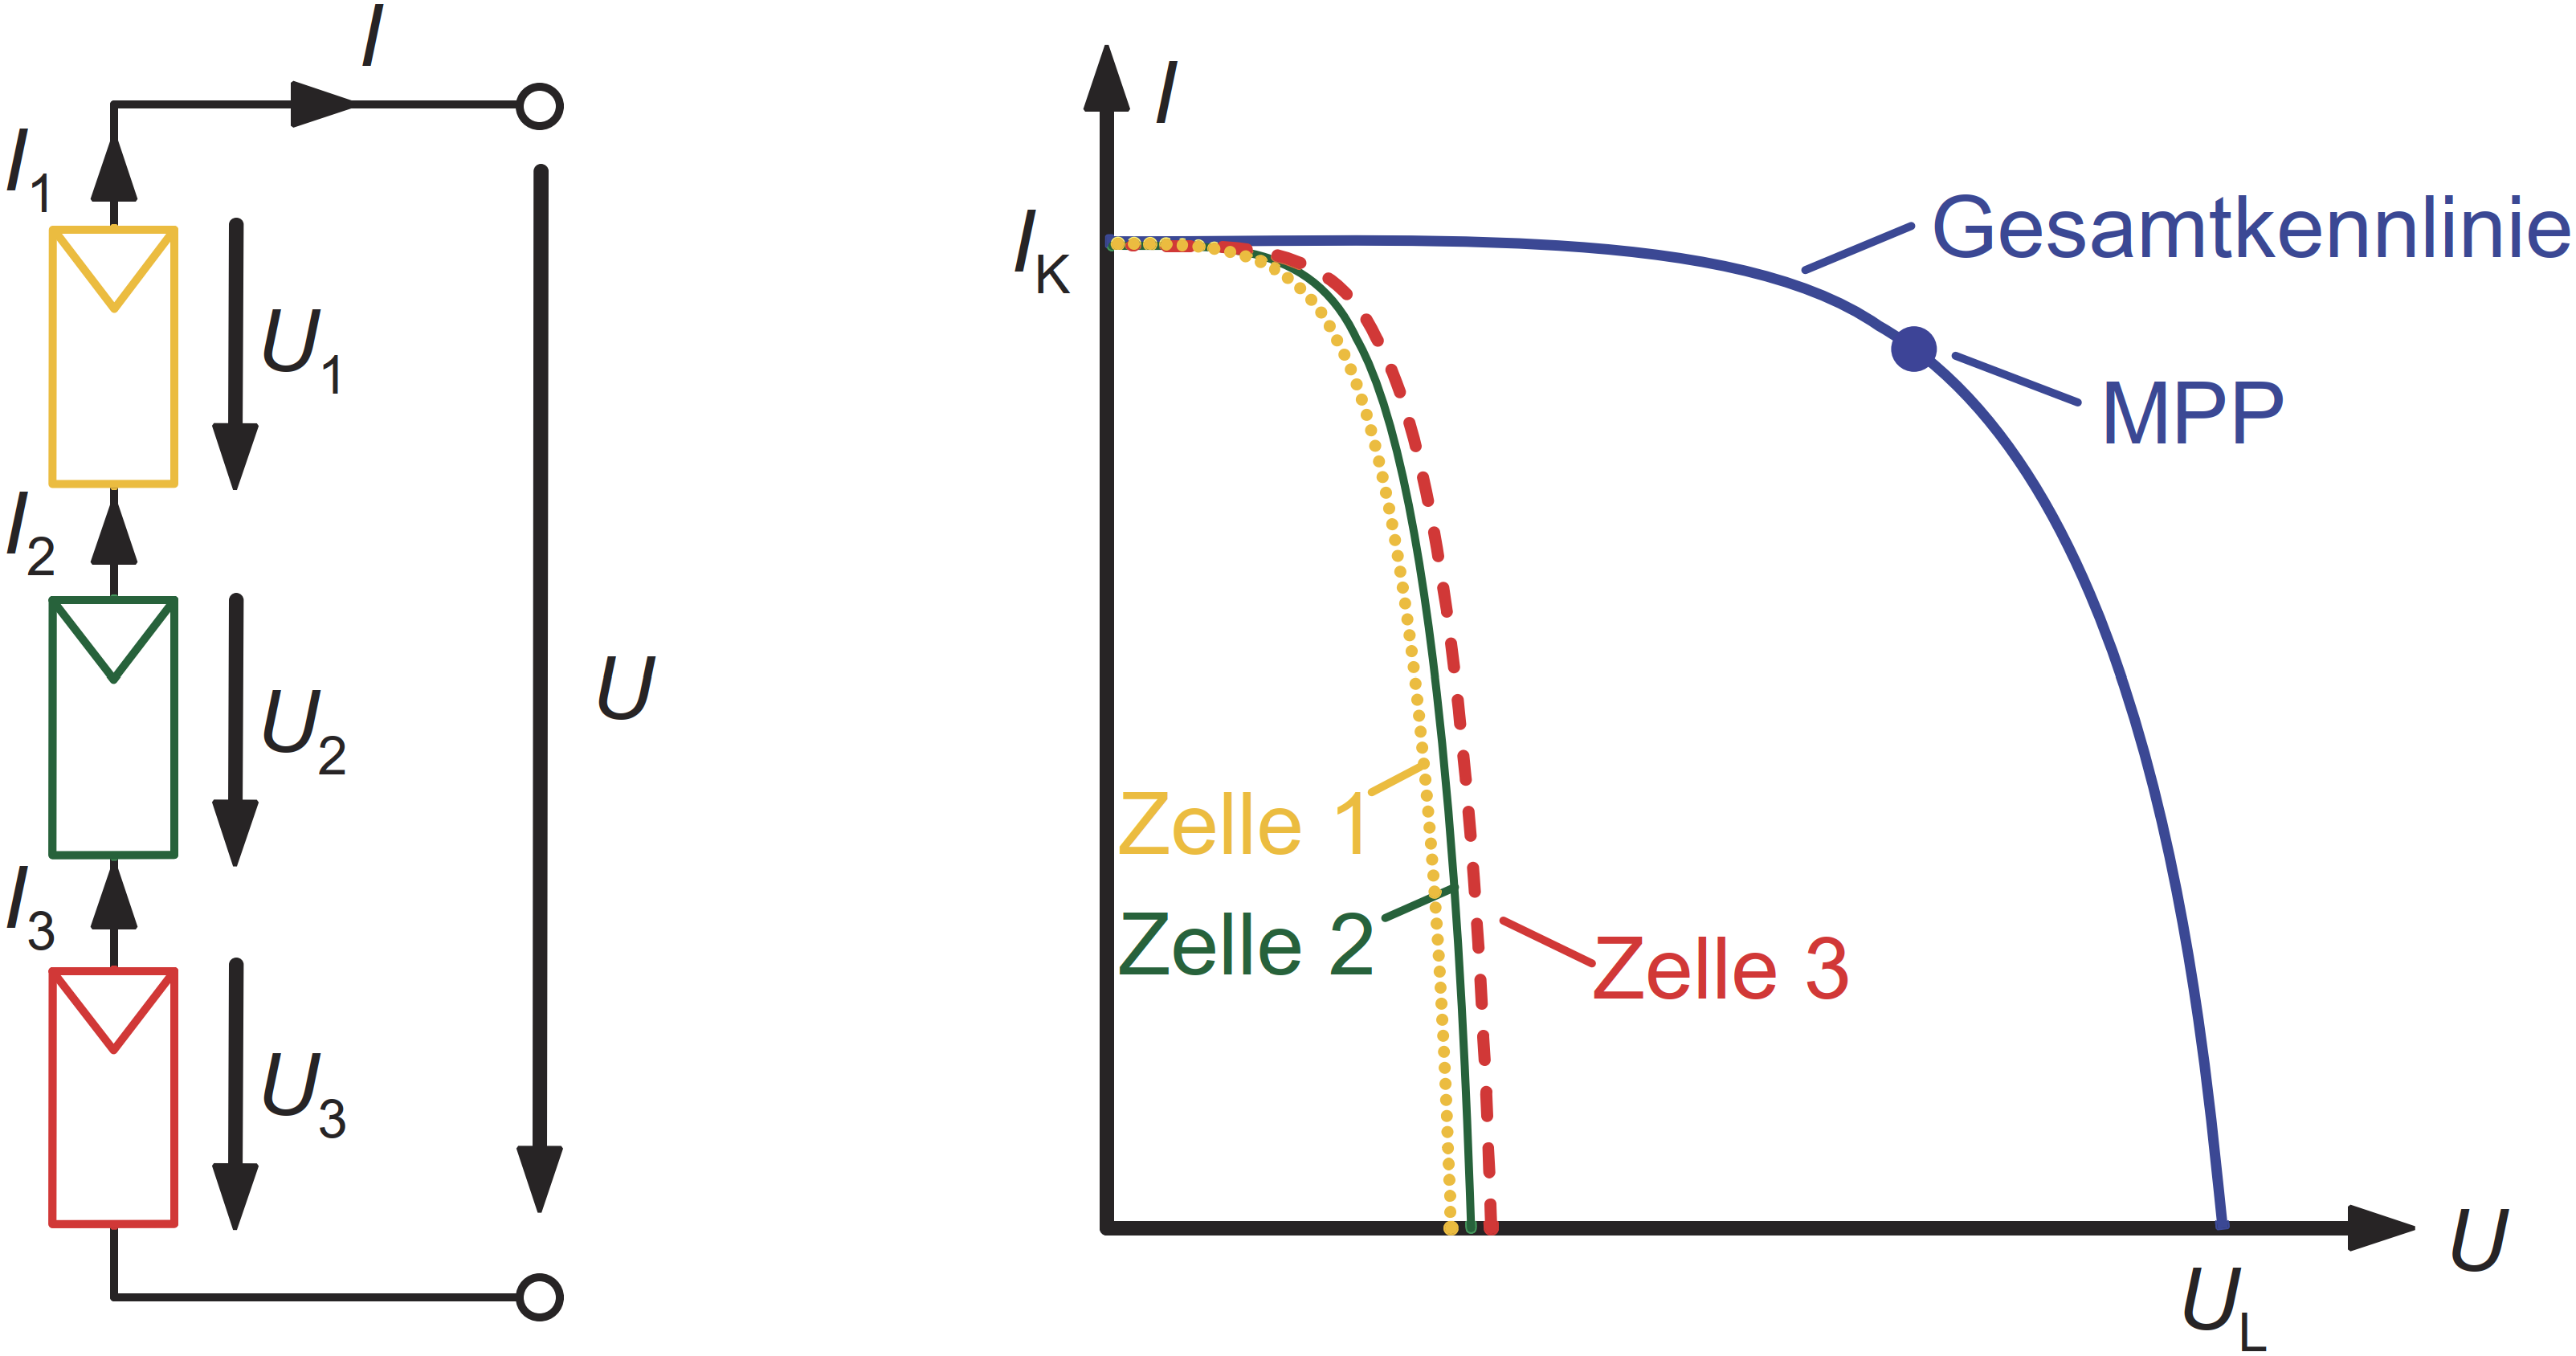
\includegraphics[width=0.7\columnwidth]{images/Serienschaltung_von_Solarzellen.png}


\subsubsection{Serienschaltung mit verschatteter Zelle}
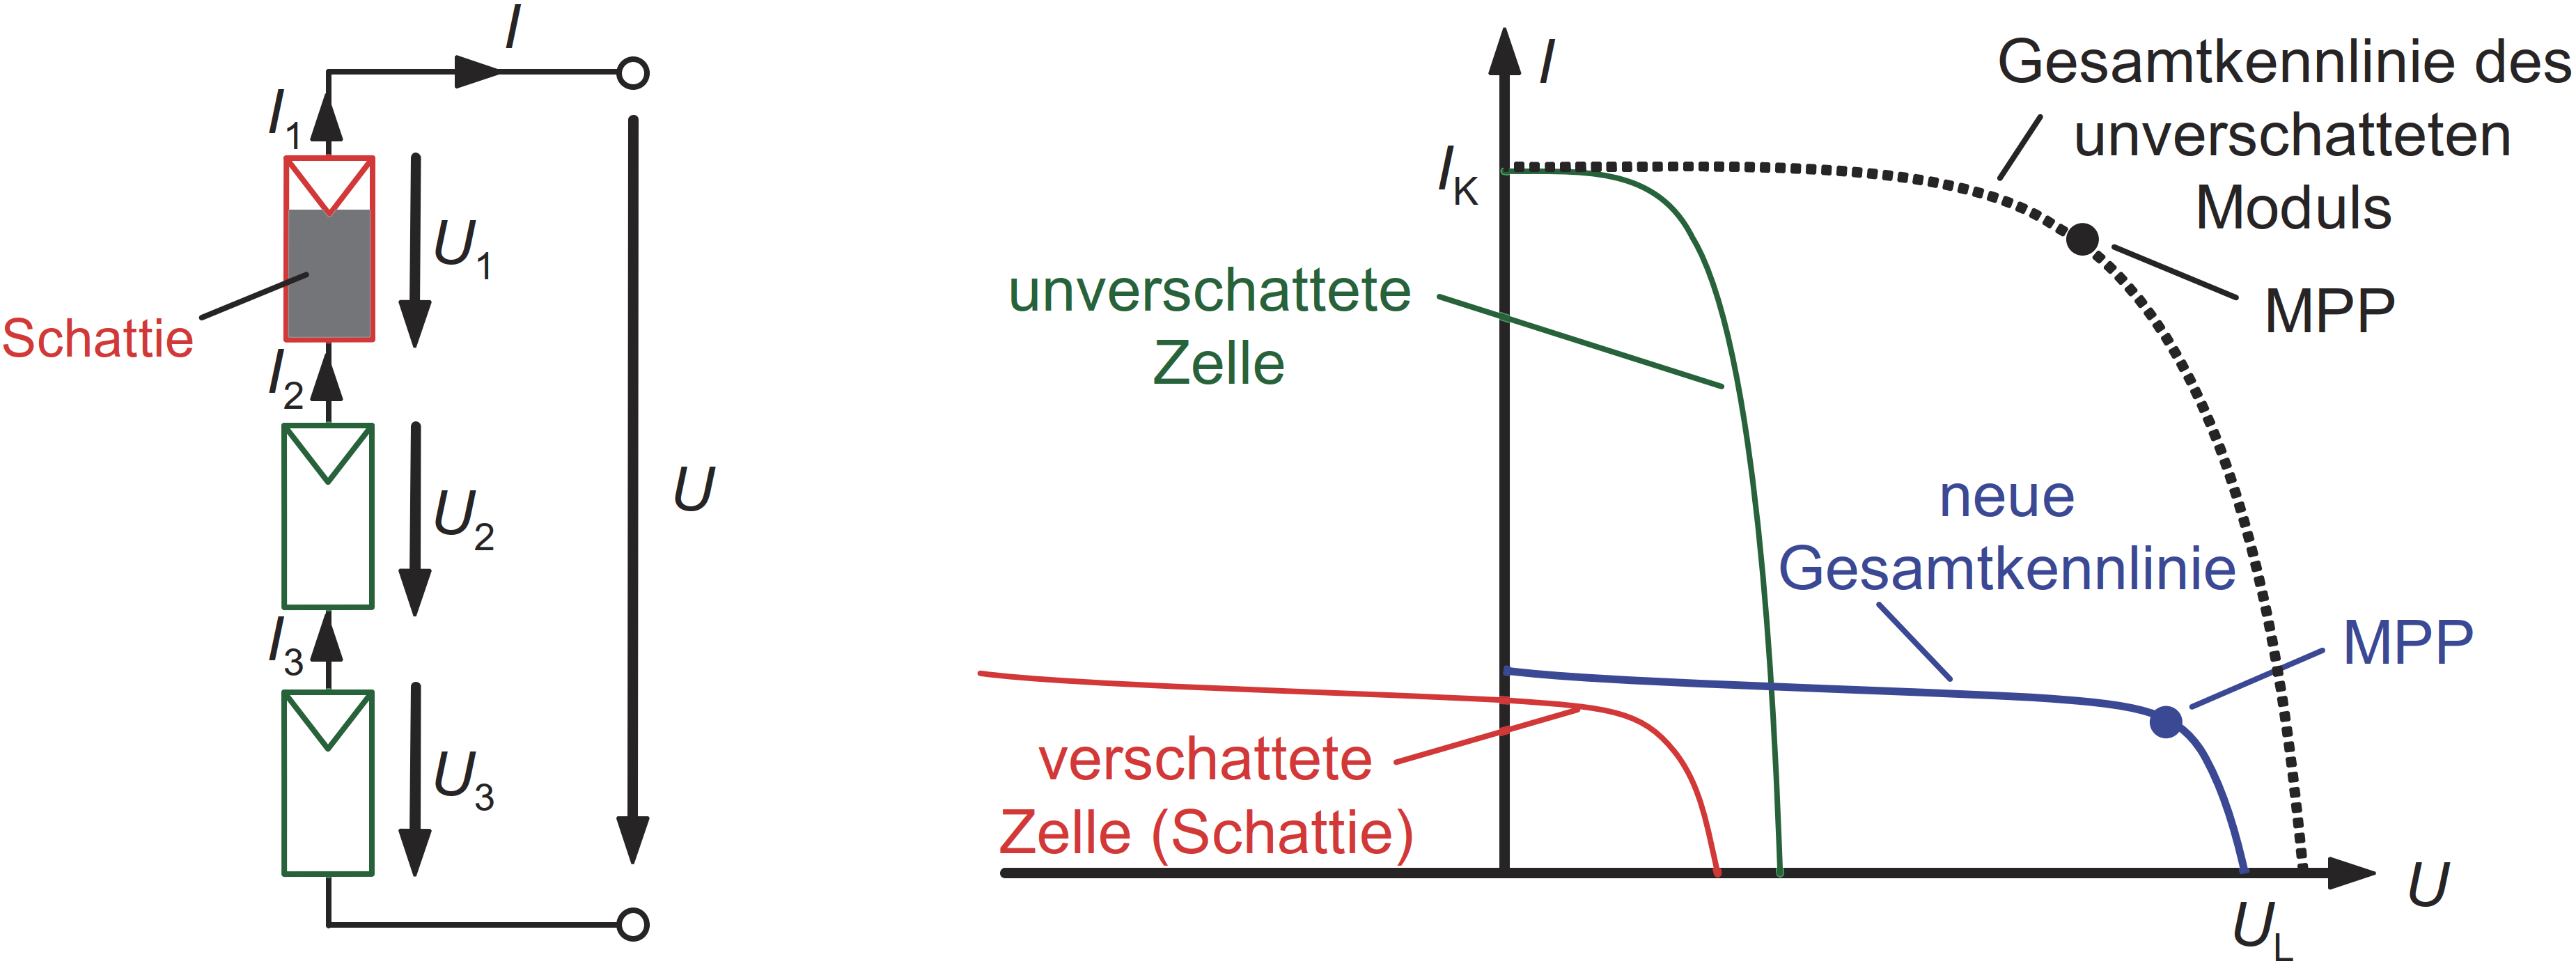
\includegraphics[width=0.98\columnwidth]{images/Serienschaltung_von_Solarzellen_mit_verschatteter_Zelle.png}


\subsection{Parallelschaltung von Solarzellen}
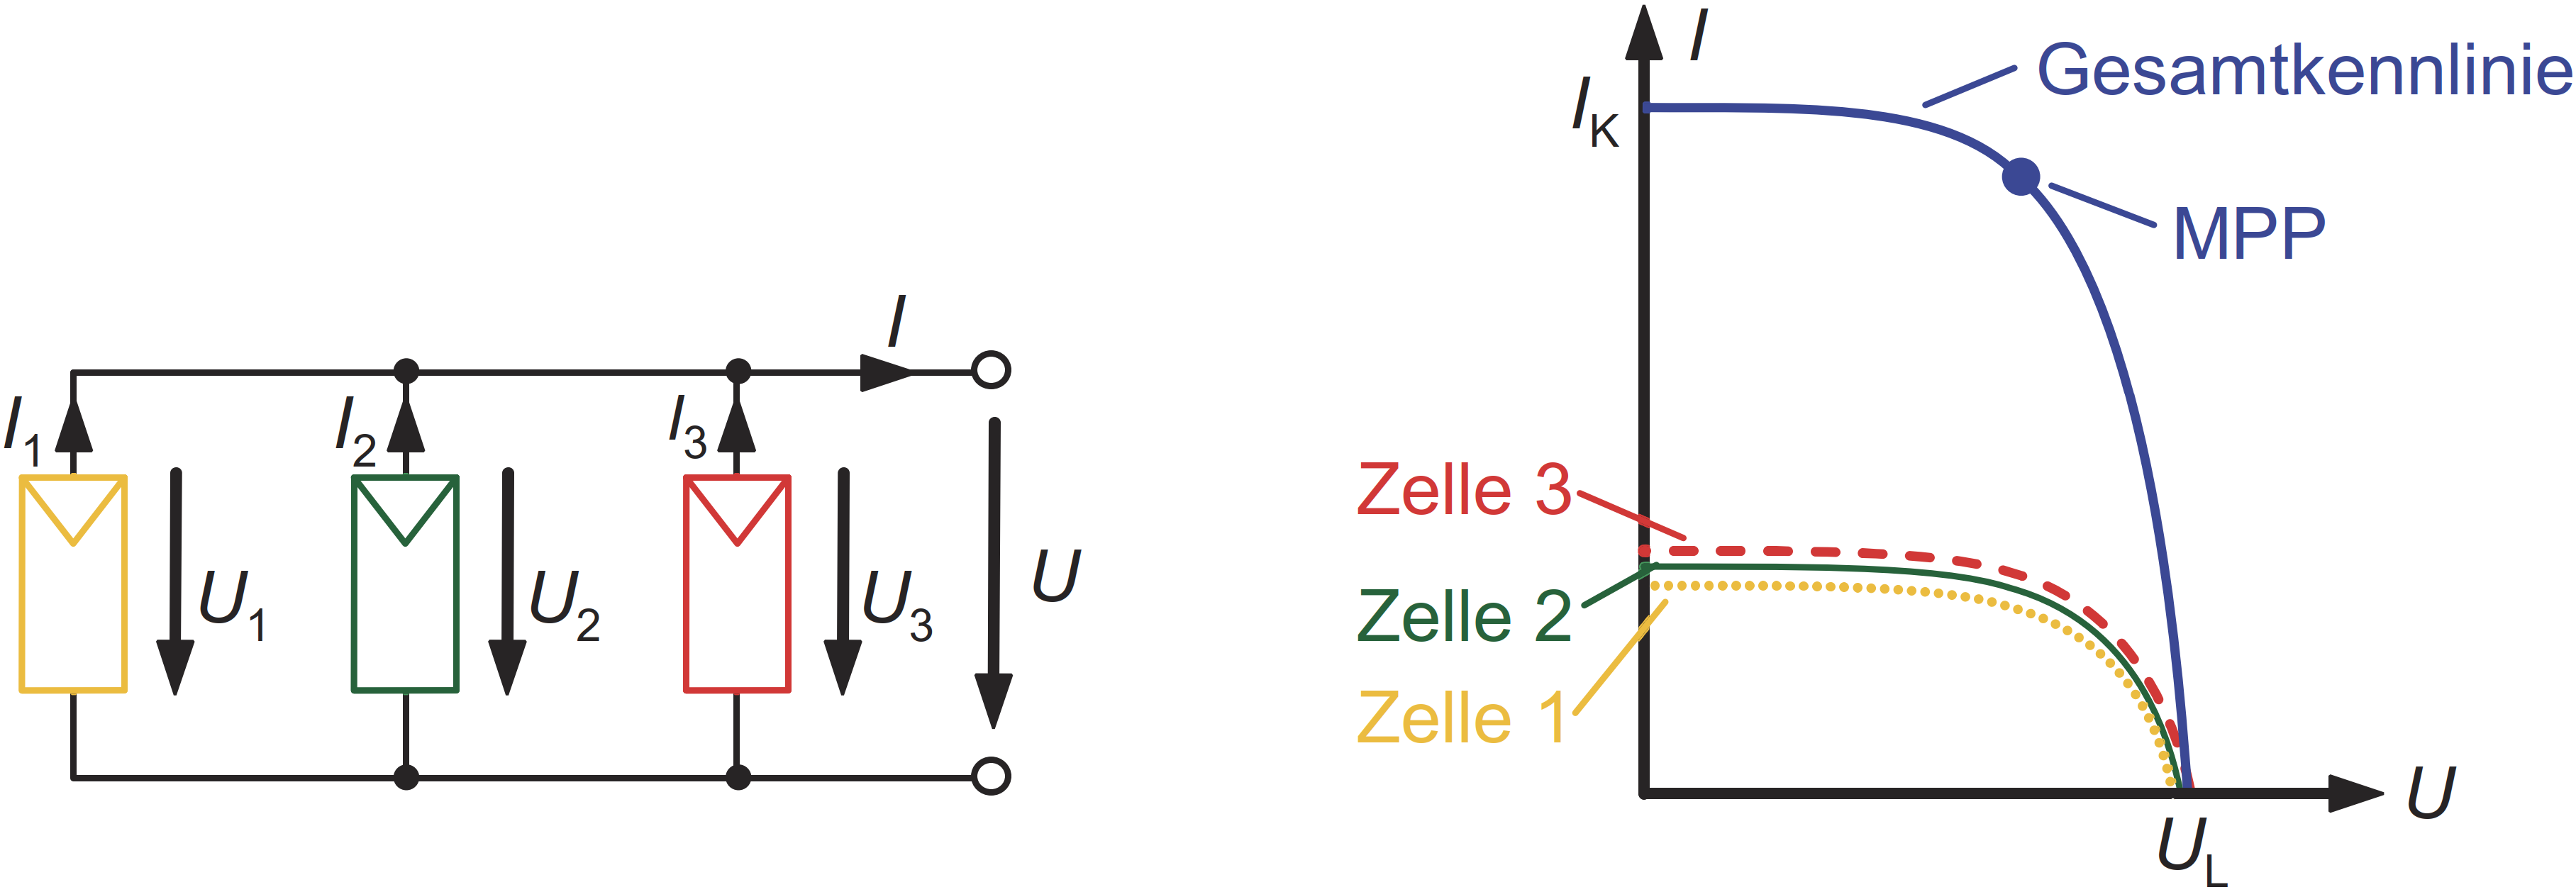
\includegraphics[width=0.95\columnwidth]{images/Parallelschaltung_von_Solarzellen.png}

\subsubsection{Parallelschaltung mit verschatteter Zelle}
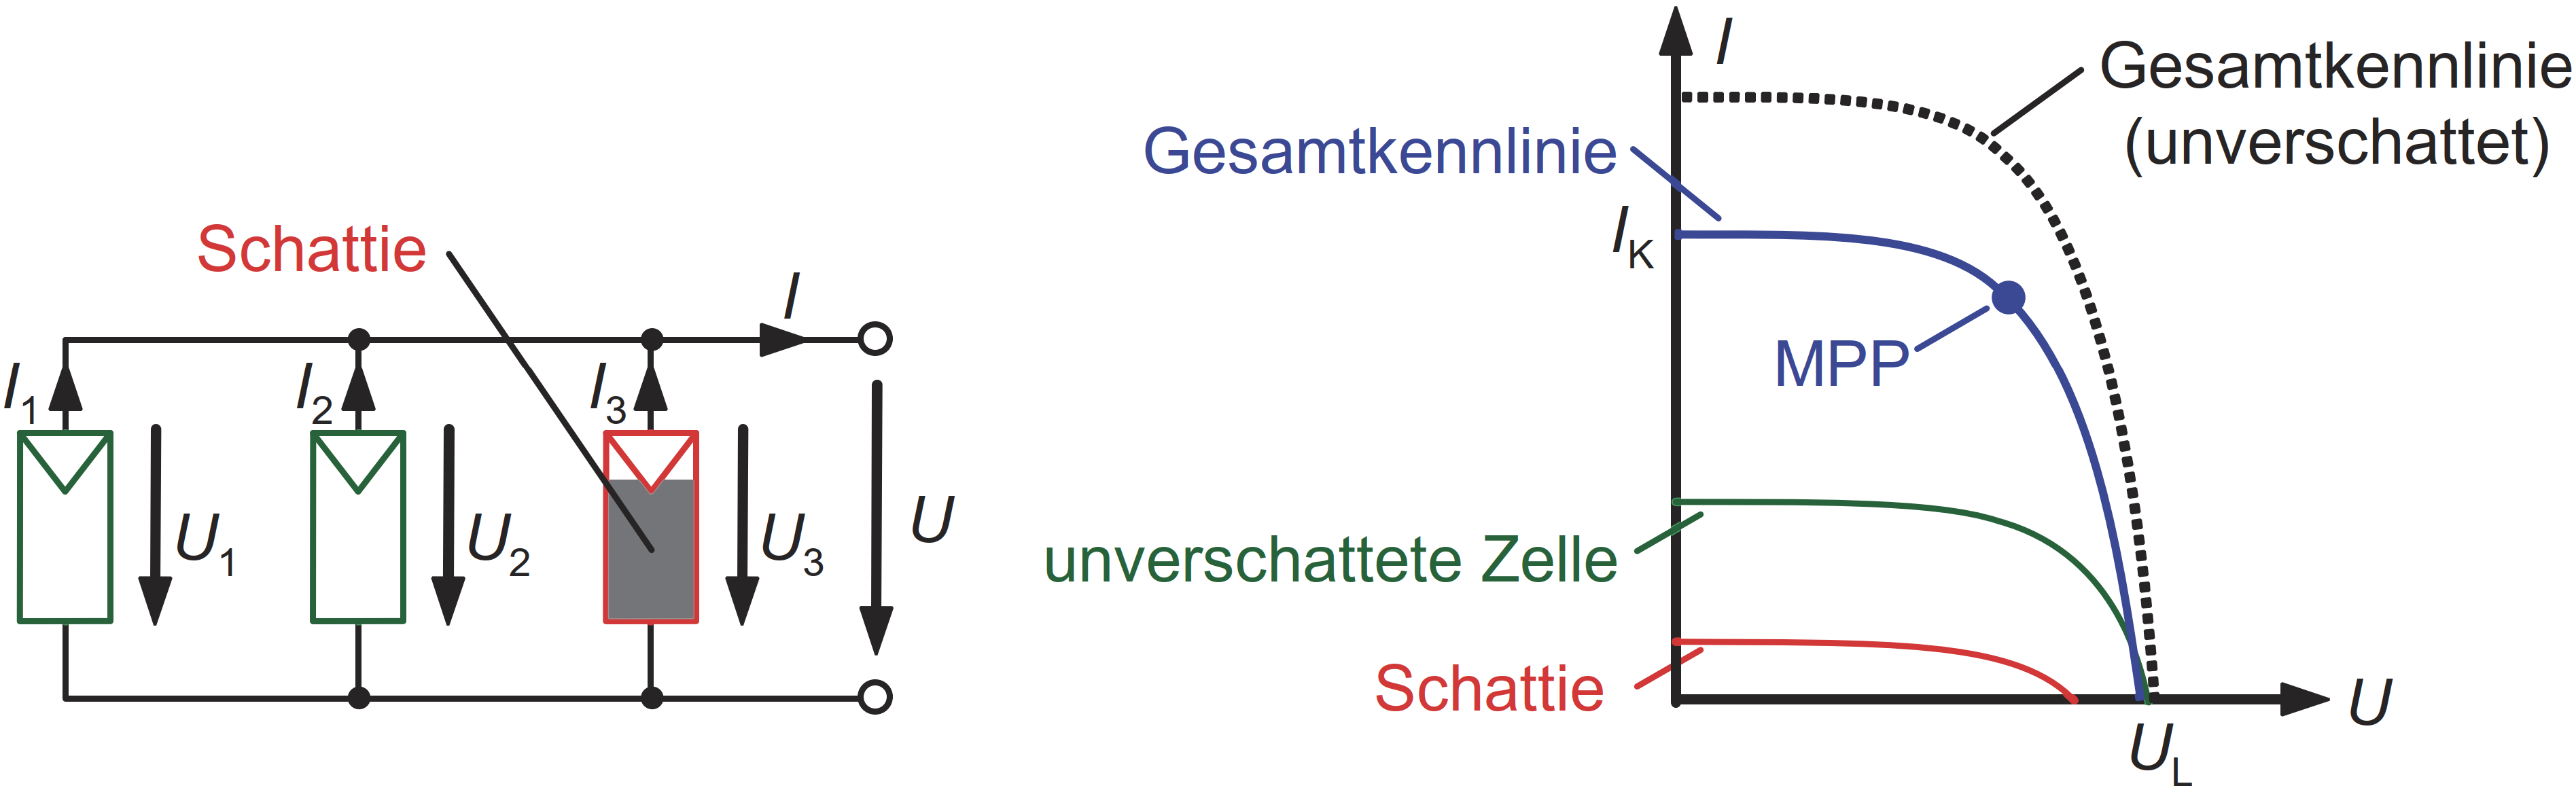
\includegraphics[width=0.95\columnwidth]{images/Parallelschaltung_von_Solarzellen_mit_verschatteter_Zelle.png}


\subsection{Beispiel aus Übungen}
Zwei Solarmodule mit den Daten \( U_L = 43{,}2\,\mathrm{V} \) und \( I_K = 10\,\mathrm{A} \) werden in Serie geschaltet. Modul A wird mit \( 1\,000\,\mathrm{W/m^2} \) bestrahlt, Modul B mit \( 500\,\mathrm{W/m^2} \). Skizzieren Sie die Einzelkurven und die Gesamtkurve für die Fälle:

\begin{enumerate}[label=\alph*.]
    \item Die Module haben keine Bypassdioden.
    \item Beide Module haben mindestens eine Bypassdiode.
\end{enumerate}

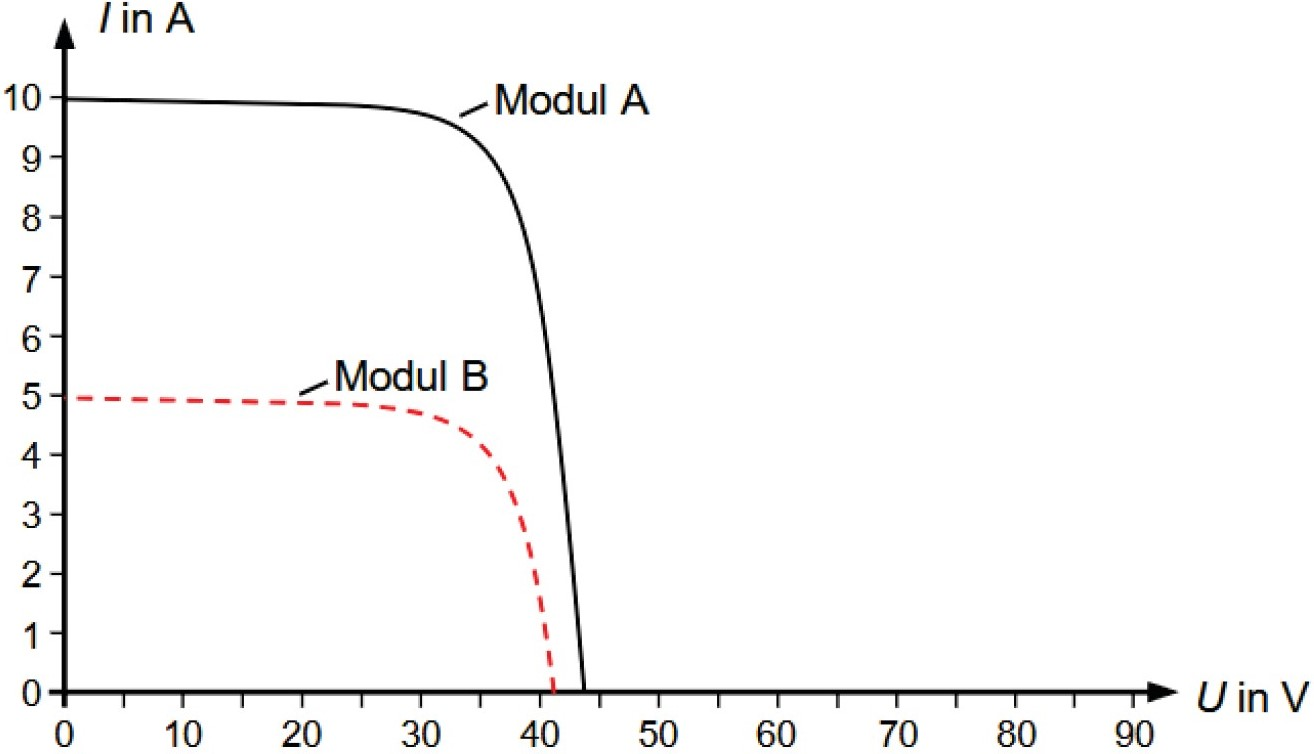
\includegraphics[width=0.6\columnwidth]{images/Beispiel_1.jpg}

\vspace{0.1cm}

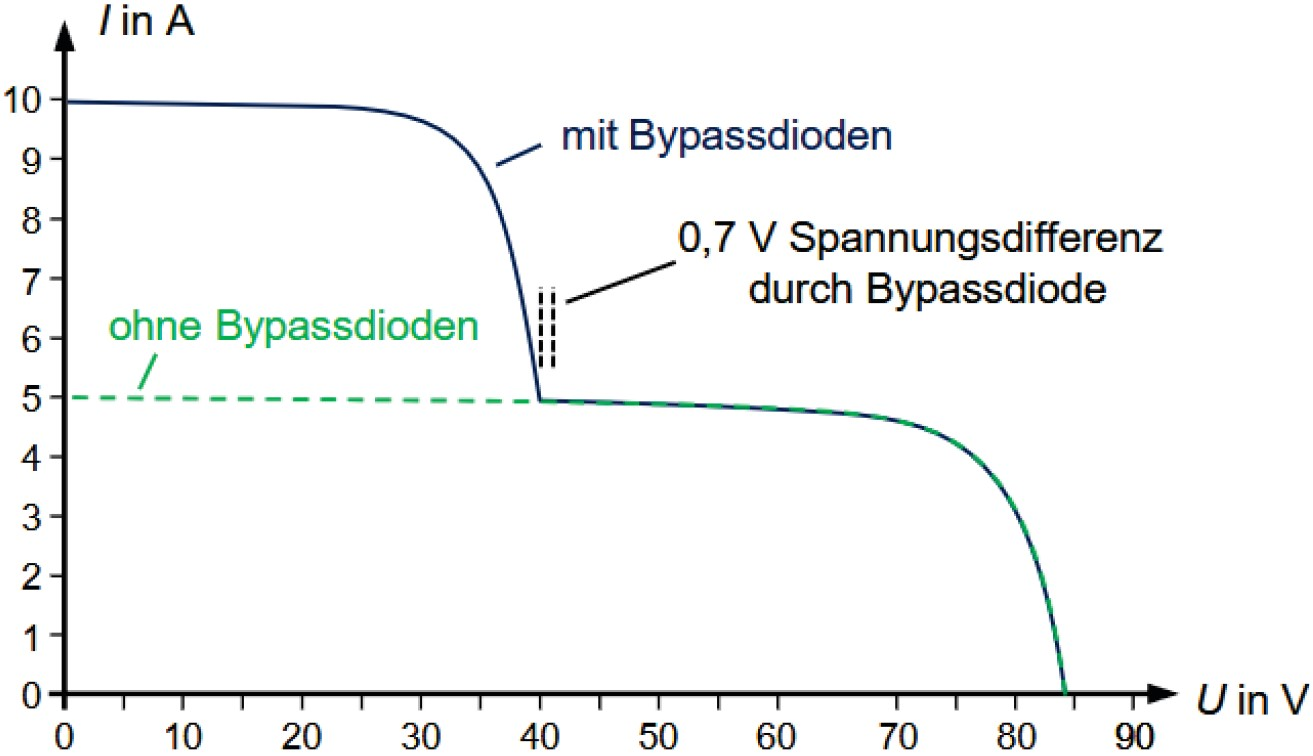
\includegraphics[width=0.6\columnwidth]{images/Beispiel_2.jpg}















